\subsection{Generische Softwareentwicklunsmodelle}
% \addcontentsline{toc}{subsection}{Generische Softwareentwicklunsmodelle}
\label{Generische Softwareentwicklunsmodelle}
Allgemein folgt jeder Prozess der Softwareentwicklung den gleichen grundlegenden Schritten. Diese werden in der nachstehenden Grafik in Anlehnung an \cite[Abb. 9.1]{Ludwig_Lichter_2013} dargestellt:

\begin{center}
    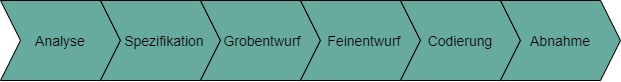
\includegraphics[width=0.8\textwidth]{Grafiken/GenerischeSchritteSoftwareentwicklung.png}
    \captionof{figure}{Generische Schritte des Softwareentwicklungsprozesses}
    \label{Grafik:Generische Schritte des Softwareentwicklungsprozesses}
\end{center}

Jede der Phasen erfüllt dabei feste Aufgaben:
% !h um die automatische Anordnung am Seitenanfang zu unterdrücken
% https://de.overleaf.com/learn/latex/Tables#Positioning_tables
% \begin{table]} ... \end{table} damit diese Tabelle im Tabellenverzeichnis aufgenommen wird
% Landscape für Querausrichtung der Tabelle
    \begin{table}[!h]
        \centering
        \begin{tabular}{|p{4cm}|p{8cm}|}
            \hline
            Phase & Aufgabe\\
            \hline
            Analyse & Aufnahme der Anforderungen an eine Software und der (Projekt-) Umgebung. \glqq{}Konkretisierung der Analyse\grqq{} \cite[S. 155]{Ludwig_Lichter_2013}\\
            \hline
            Spezifikation & Präzisierung / Verschriftlichung der Analyse\\
            \hline
            Grobentwurf & Festlegung der groben Programmstruktur\\
            \hline
            Feinentwurf & Präzisierung des Grobentwurfs, Festlegung der genauen Implementierung\\
            \hline
            Codierung & Umsetzung des Feinentwurfs in Code, Tests des Codes (Unit-Tests)\\
            \hline
            Integration, Test und Abnahme & Einpassung des Produktes in die Produktivumgebung\\
            \hline
        \end{tabular}
            \caption{Generische Phasen der Softwareentwicklung}
            \label{Generische Phasen der Softwareentwicklung}
    \end{table}

Diese Phasen sind in sich abgeschlossen und haben definierte Übergabepunkte (Artefakte) bei einem Wechsel zwischen zwei Phasen \cite[S. 155]{Ludwig_Lichter_2013}. Hierzu sei erwähnt, dass es sich um eine vereinfachende und idealisierte Betrachtung handelt. Der feste \textit{Top-to-Bottom}-Ansatz ist für die meisten praktischen Anwendungsfälle zu simpel und wird veränderbaren oder wechselnden Anforderungen nicht gerecht. Diese Einschränkung hat bereits  Dr. Winston W. Royce als Erfinder des Wasserfallmodells \cite{royce1987managing} erkannt und ihr Rechnung getragen. Royce selbst hat eine Wiederholung der Modelldurchläufe vorgeschlagen \cite{Larmann_Basili_2003} und damit das lineare Modell iterativ erweitert. Die nachstehende Grafik verdeutlicht dies in Anlehnung an \cite[Abb. 3]{royce1987managing}:

\begin{center}
    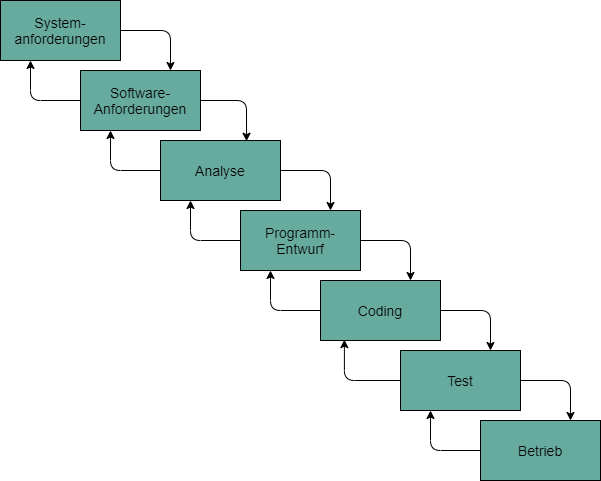
\includegraphics[width=0.8\textwidth]{Grafiken/IterativesWasserfallmodell.png}
    \captionof{figure}{Iteratives Wasserfallmodell nach Royce}
    \label{Grafik:Iteratives Wasserfallmodell nach Royce}
\end{center}

Ein iterativer Ansatz ermöglicht es, auf Veränderungen interner und externer Faktoren in einem Softwareprojekt zu reagieren. Dabei ist es zunächst unerheblich, welche Faktoren dies sind (Entweder externe, wie z.B. veränderte Anforderungen oder interne, wie z.B. Wechsel einer Programmierungsmethode). Entscheidend ist nur die Phase, in welcher die Veränderungen auftreten. An diesem Punkt kann die einzelne Phase (oder alle bis dahin durchlaufenen Phasen) erneut durchlaufen werden. Dieser lineare Ablauf wird im Spiralmodell weiter erweitert:

\begin{center}
    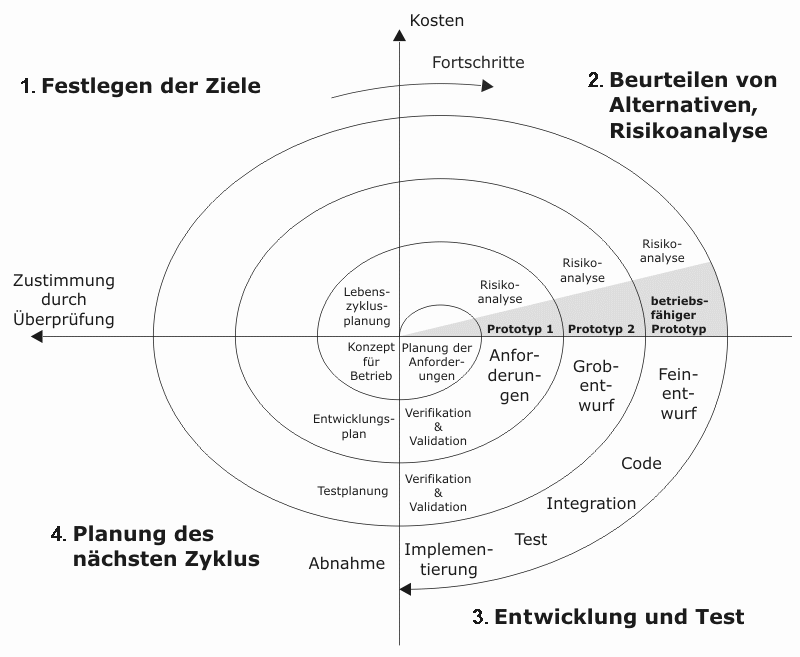
\includegraphics[width=0.8\textwidth]{Grafiken/Spiralmodel_nach_Boehm.png}
    \captionof{figure}{Spiralmodell nach Boehm \cite[Abb. 2]{boehm_spiral_1988}, Grafik aus \cite{wikipedia_spiralmodell_2004}}
    \label{Grafik:Spiralmodell nach Boehm}
\end{center}

Von diesen Modellen können weitere Formen abgeleitet werden. Daher werden sie als generische Entwicklungsmodelle bezeichnet.